\chapter{Experimental Setup}

This chapter will discuss the experimental setup for studying heavy ion collisions and QGP. We will start by describing the RHIC accelerator at BNL. We also examine the STAR detector, triggering, data acquisition, and its particle identification capabilities. We will talk in greater detail about the detector subsystems which are most relevant to the identification of electrons from heavy flavor processes. 

\section{Relativistic Heavy Ion Collider}

The Relativistic Heavy Ion Collider (RHIC) is an accelerator facility located at Brookhaven National Lab which was built for the study of QCD at high temperatures as well as probing the spin structure of protons. The collider is capable of colliding a variety of heavy nuclei (to date: gold, uranium, and copper) as well as lighter particles (protons, deuterons, and recently helium-3). RHIC is also capable of colliding polarized proton beams for the program studying the spin structure of the proton. The top energy for collisions at RHIC is 500 GeV for p+p and 200 GeV per nucleon for Au+Au. 

The main collider rings at RHIC are 2.4 miles in circumference and intersect at six interaction points. Particles are brought up to collision energies through a series of linear accelerators and booster synchrotrons~\cite{RHICacc}. Figure~\ref{fig:RHIC} shows the layout of the RHIC facilities as well as the location of some experiments that have run or are currently running at RHIC. PHENIX and STAR are the two long running general purpose detectors at RHIC.

\begin{figure}[htbp]
\begin{center}
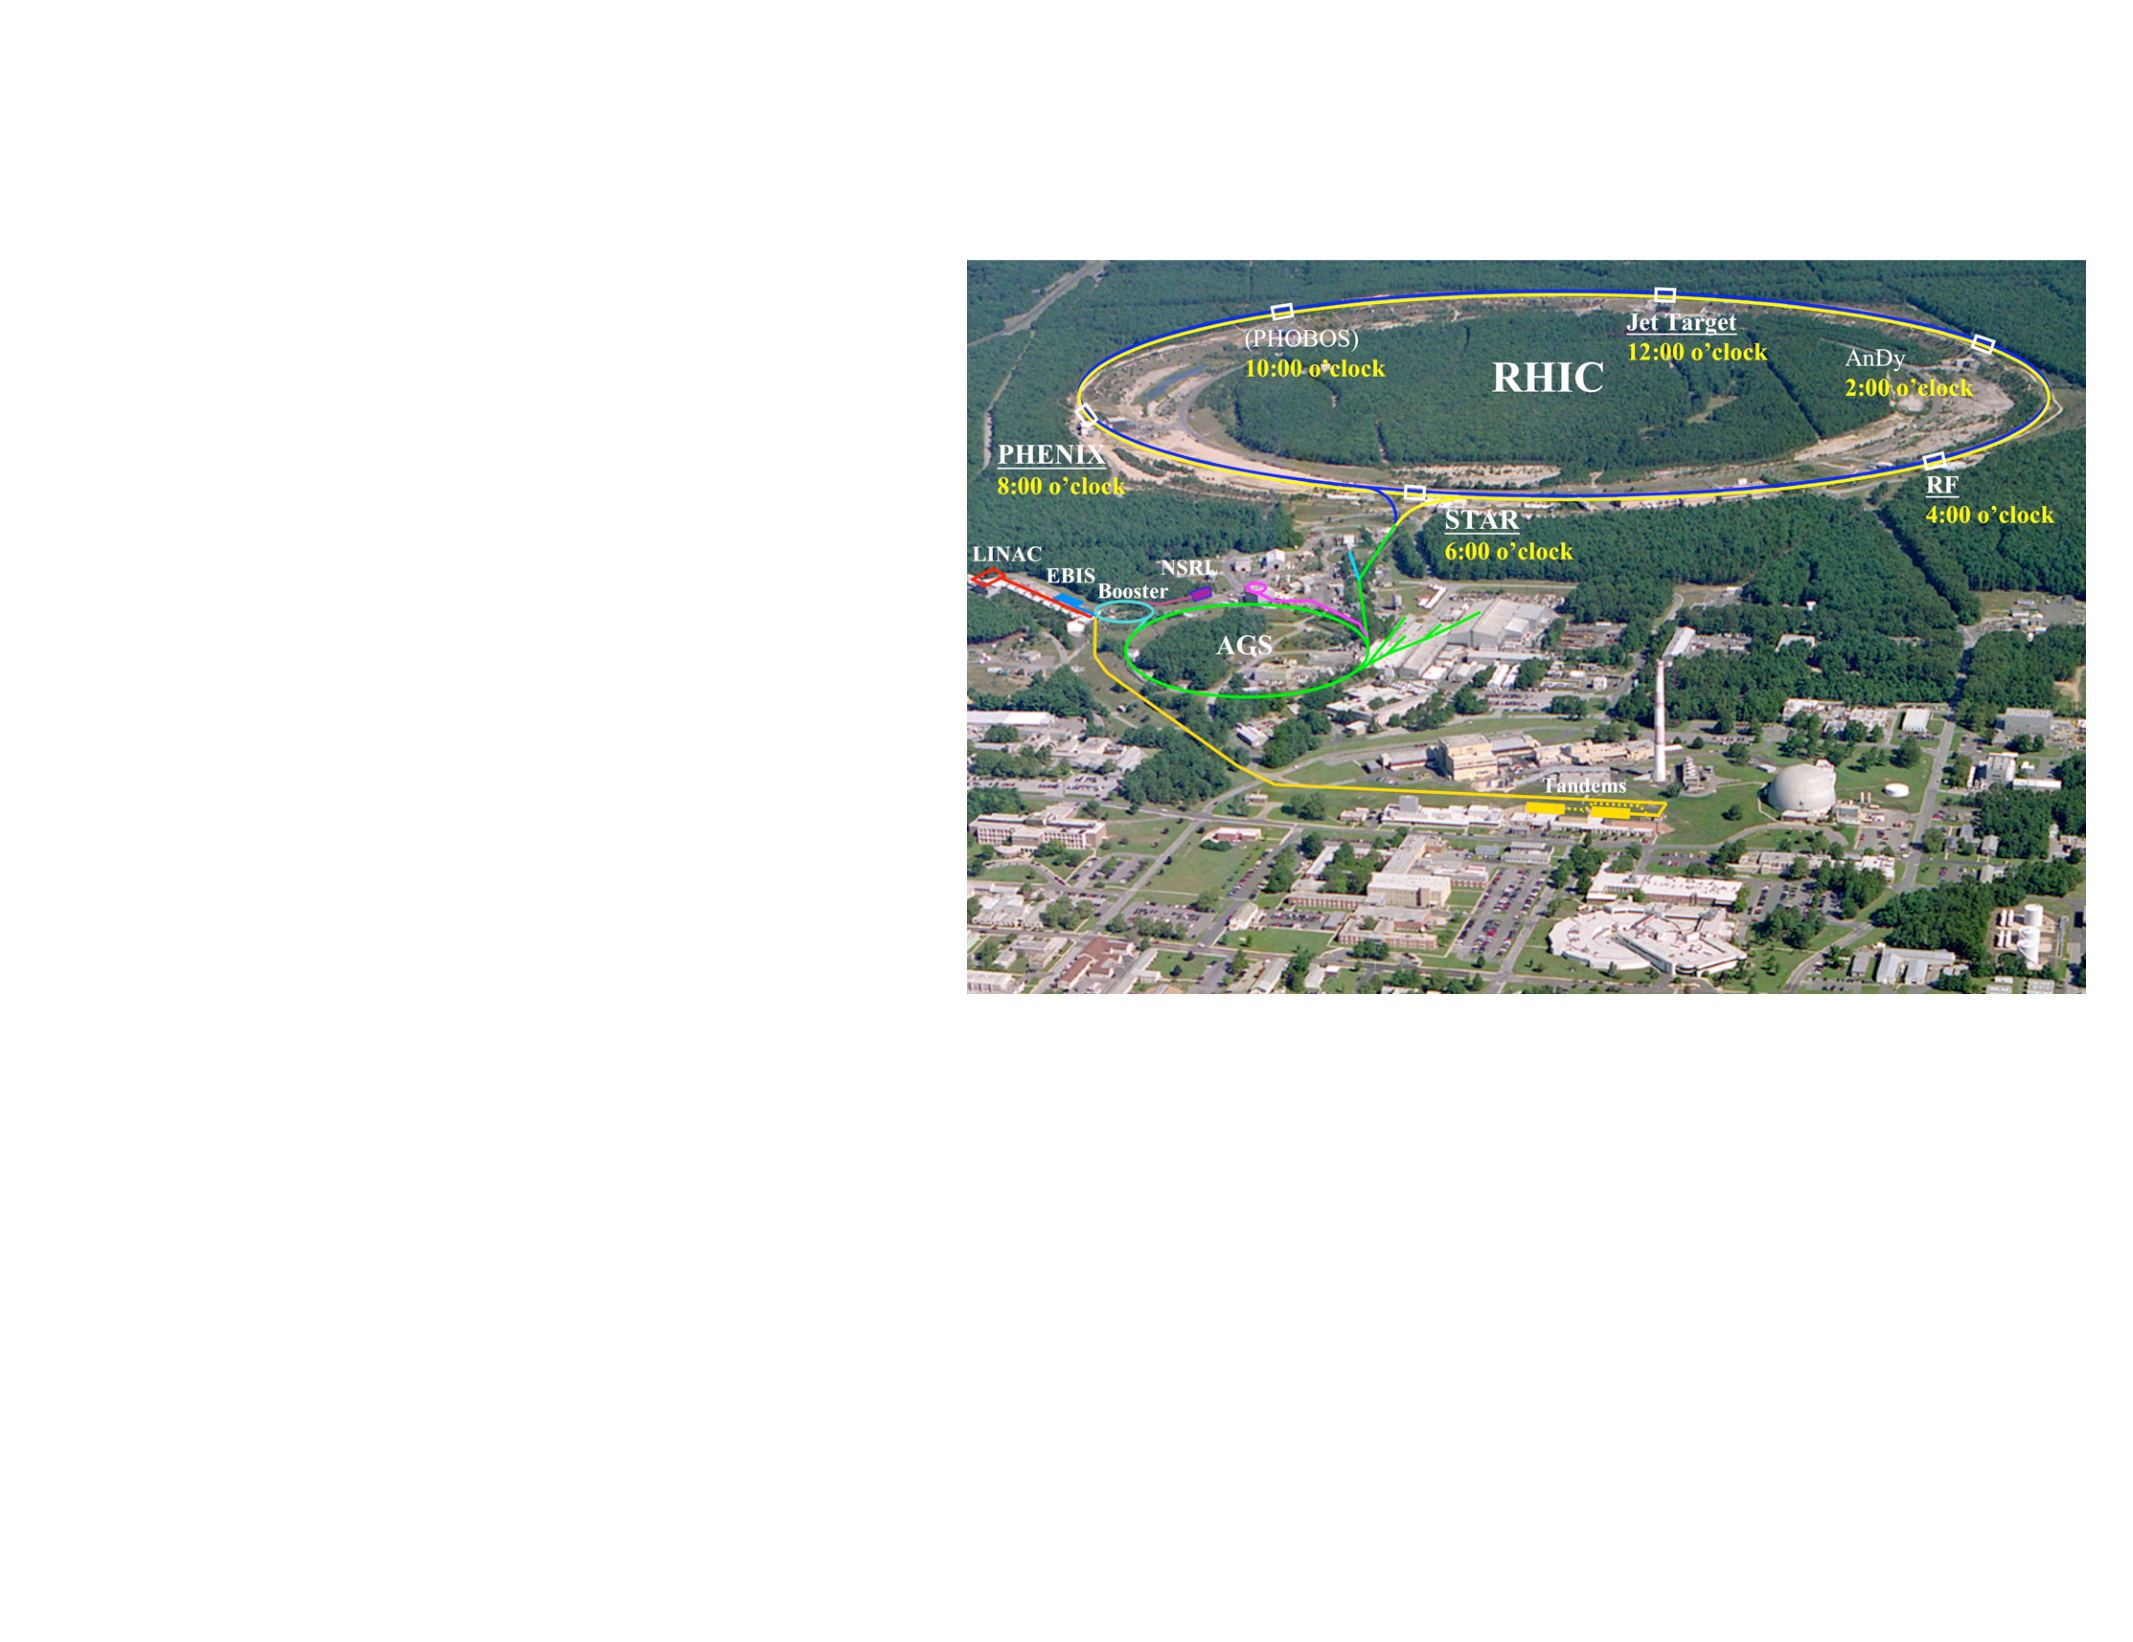
\includegraphics[scale=0.75]{Plots/Detector/RHIC_Complex.pdf}
\end{center}
\caption[RHIC Facility]{RHIC Complex seen from above. Top of the picture shows the main rings and locations of various experiments. Lower part shows the LINAC and AGS. Picture from~\cite{RHICpic}.}
\label{fig:RHIC}
\end{figure}

For the run in 2011 gold nuclei were generated from an ion source and then initially accelerated in the Tandem Van de Graff line. RHIC had multiple Van de Graff accelerators allowing for collisions between mixed nuclei (for example, Au+Cu or d+Au). From 2012 onwards, the function of the tandems was replaced by the Electron Ion Beam Source (EBIS) which generates particles from deuterons to uranium nuclei. Proton beams on the other hand originate from the 200 MeV LINAC. Both protons and other nuclei move to the booster synchrotron which further accelerates the particles using RF waves. After passing through the booster ring the beams then enter the Alternating Gradient Synchrotron (AGS). The AGS was a long running and highly successful facility at BNL, three Nobel Prizes resulted from research conducted at AGS. Now AGS serves as a final booster ring before sending the beams to the main RHIC rings. 

The beams then reach RHIC where the last remaining electrons are stripped away leaving only the nuclei. In the storage rings the particles circulate in bunches, typically around 110 bunches per ring, and the beams are brought to their collision energy. The beams can collide at six interaction points along the ring. Top energy for the heavy ion program in 200 GeV per nucleon, higher energies are used in some p+p collisions and RHIC is also capable of colliding at lower energies as is the case in the beam energy scan program which explores the QCD phase diagram.

\section{STAR Detector}

The Solenoidal Tracker at RHIC (STAR) is a general purpose detector located at the 6 o'clock interaction point at RHIC. STAR consists of a variety of detector subsystems which cover a large acceptance region and allow for a variety of physics programs. This analysis will focus only on data taken with STAR's mid rapidity detectors. Figure~\ref{fig:STAR} is a schematic showing the configuration of STAR. It should be noted that for the data taking for this analysis the Silicon Vertex Tracker (SVT) was removed and only its support structure remained.

\begin{figure}[htbp]
\begin{center}
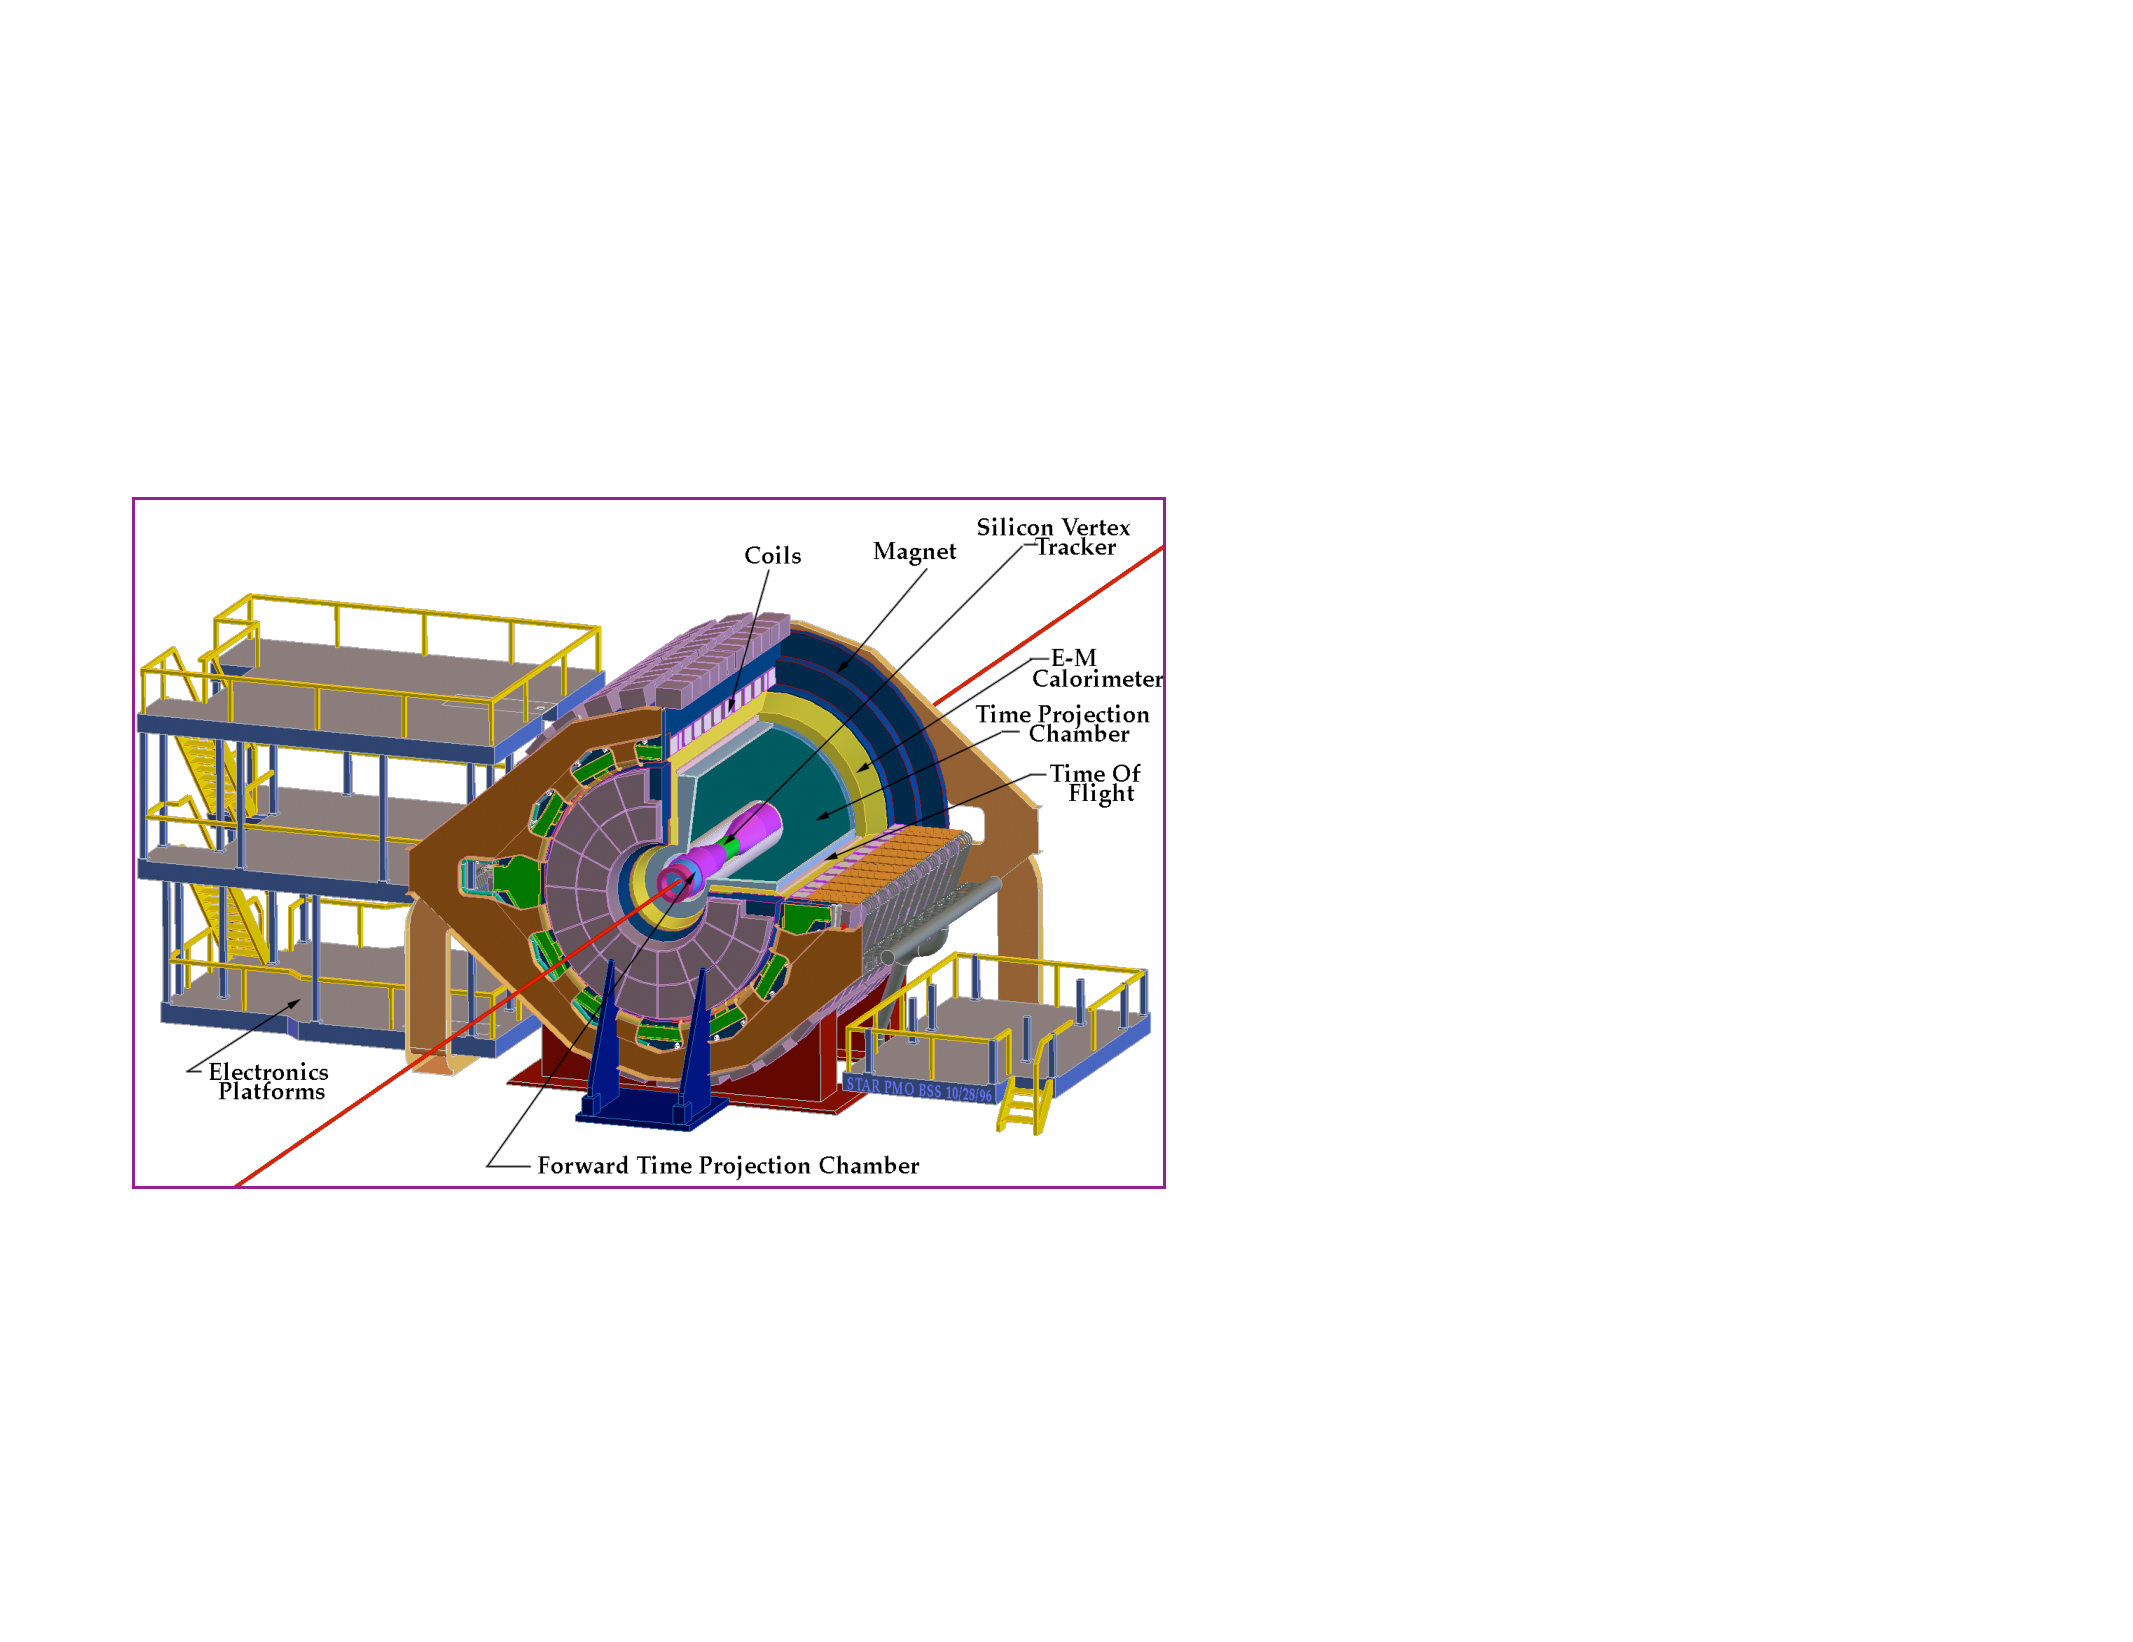
\includegraphics[scale=0.7]{Plots/Detector/STAR_Detector.pdf}
\end{center}
\caption[STAR Detector]{The STAR detector as it was configured around the time of the data taking for this analysis with the exception of the SVT which was removed prior to run 10~\cite{STARweb}.}
\label{fig:STAR}
\end{figure}

In STAR the primary tracking detector is the Time Projection Chamber (TPC) which surrounds the beam pipe, covering $2\pi$ in azimuth and capable of tracking particles in pseudorapidity up to around $\eta \approx 1.3$~\cite{tpcNIM}. The TPC can also measure ionization energy loss of charged particles, which is used for particle identification (Figure~\ref{TPC_dedx}). For runs 10 and 11 the TPC was the inner most tracking detector in STAR. Prior to this the SVT was in place as a tracking detector and from 2014 onwards the inner tracking in STAR has been upgraded with the Heavy Flavor Tracker (HFT) which is capable of improving resolution on secondary vertices. Outside of the TPC is the Time of Flight (TOF) detector~\cite{vpdNIM}. TOF greatly improves the particle identification for low momentum hadrons. Further outside of TOF and the TPC is the Barrel Electromagnetic Calorimeter (BEMC), consisting of a lead-scintillator sampling calorimeter and Shower Maximum Detector (SMD). The BEMC allows for measurements of electron energies, improves the identification of high $p_T$ electrons, and allows for identifying $\gamma$'s which cannot be tracked in the TPC. Sitting outside the BEMC is the Muon Telescope Detector (MTD) which can be used for the measurement of $J/\psi$ decays through the di-muon channel. For measurements of non-photonic electrons we use the tracking and PID from the TPC as well as additionally PID information from the BEMC systems.

\section{Time Projection Chamber}

The TPC is the main tracking and particle identification system in STAR, it surrounds the beam pipe and interaction region and has full azimuthal coverage and covers $\pm 1.8$ in pseudorapidity~\cite{tpcNIM}. The TPC is a cylindrical volume, 4.2 m long, with an inner diameter of 1 m and an outer diameter of 4 m. The enclosed volume is filled with a mixture of 10\% methane and 90\% argon. The TPC sits inside of the STAR solenoid magnet which is capable of producing magnetic fields of .5 T in two opposite polarities. Bending of tracks of charged particles in the TPC allows for tracking of particles from .1 GeV/c to 30 GeV/c. Midway down the length of the TPC the chamber is divided by the Central Membrane. A potential is established between the Central Membrane, the cathode, and the end caps of the TPC, the anodes. Inner and Outer Field Cages run the length of the TPC along the walls, gradually increasing in potential as they get closer to the Central Membrane. The field cages help establish a uniform electric field in the TPC which is critical for tracking resolution. Figure~\ref{fig:TPC} shows an illustration of the TPC and the locations of the Central Membrane and field cages.

\begin{figure}[htbp]
\begin{center}
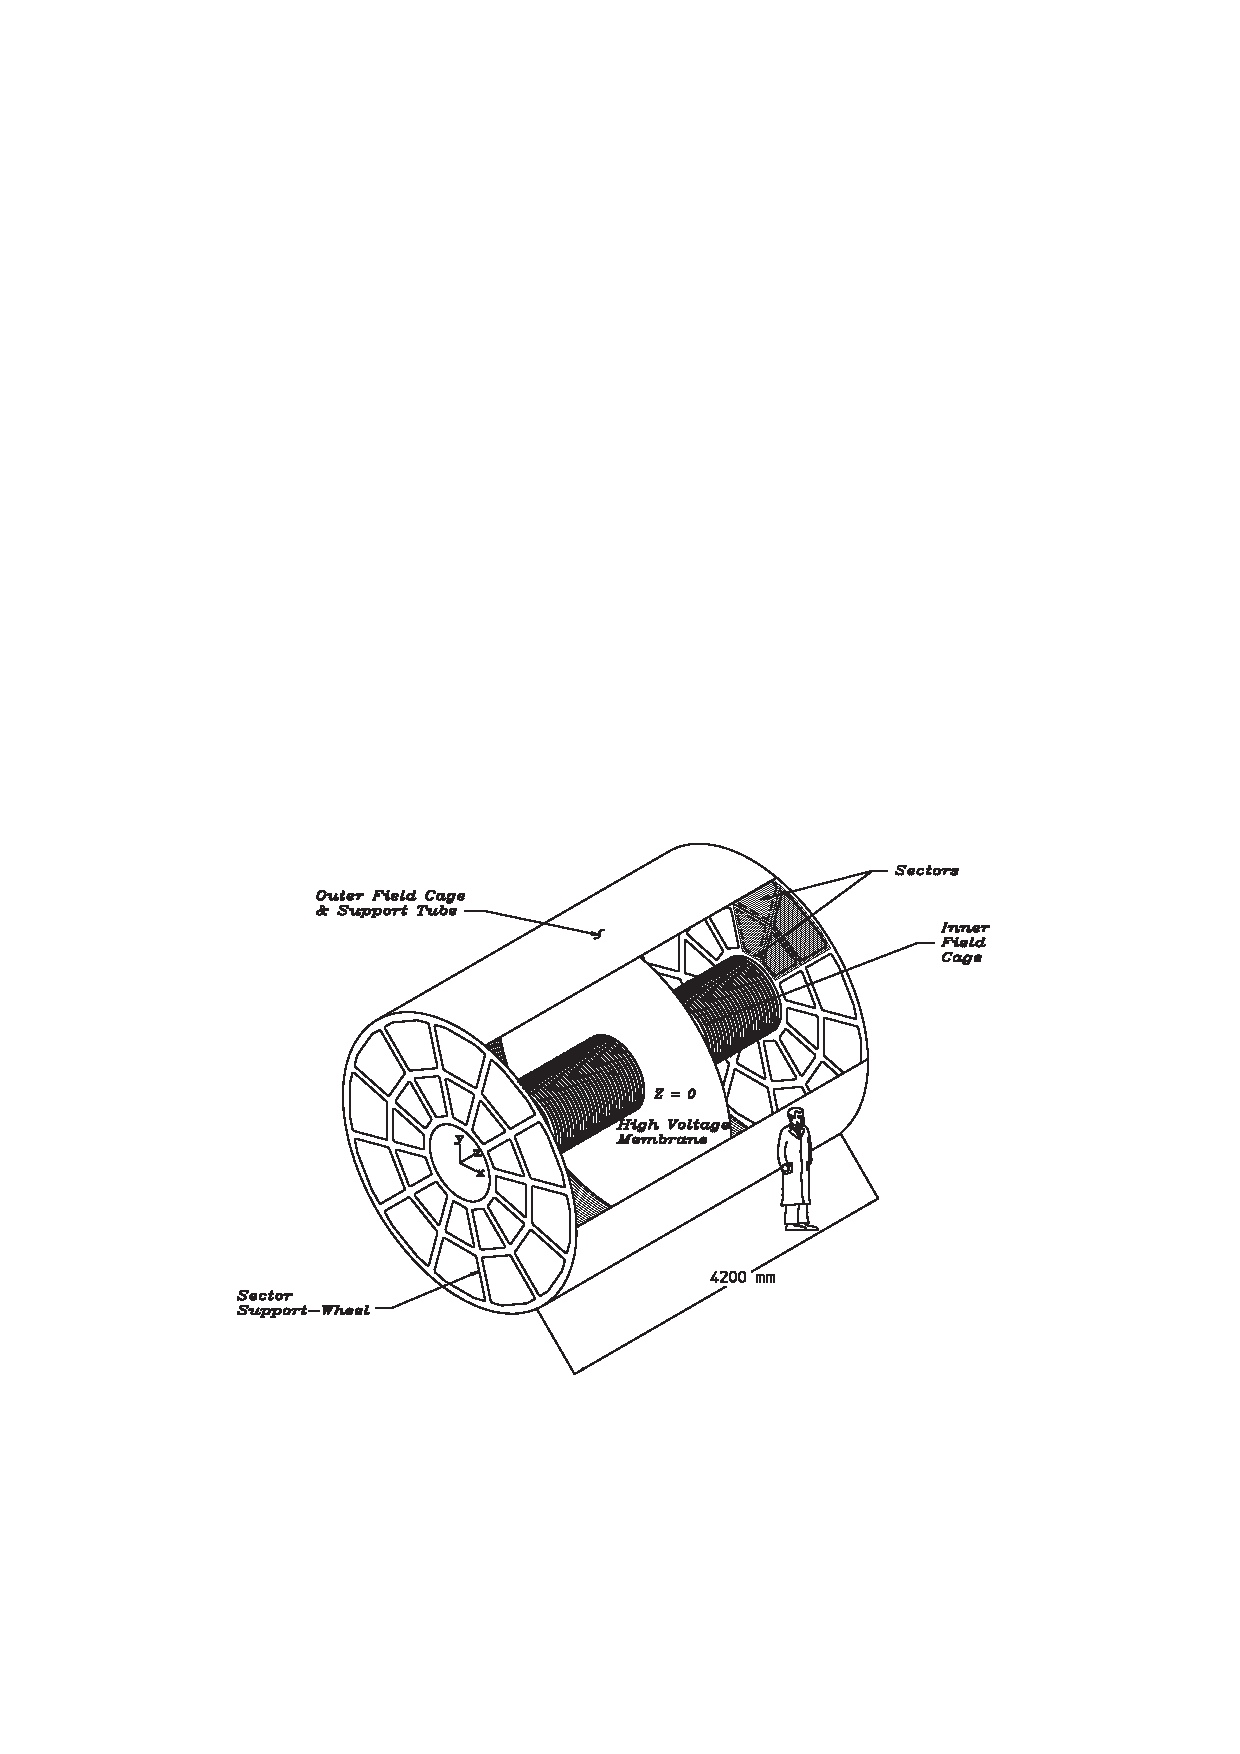
\includegraphics[scale=1.0]{Plots/Detector/TPC.pdf}
\end{center}
\caption[TPC Diagram]{Diagram of the STAR TPC showing the main components as well as the scale. From~\cite{tpcNIM}}
\label{fig:TPC}
\end{figure}

Charged particles traverse the TPC and ionize the gas inside. The electrons inside it drift along the electric field in the TPC at 5.45 cm/$\mu$s towards the ends of the TPC where the readout pads are located. The endcaps of the TPC chambers are divided radially into 12 sections, each section has an inner and outer segment (Figure~\ref{fig:TPC_pad}). The TPC readout sectors have 4 components, a pad plane and three wire planes. The outermost wire plane is a gating grid which can block ions from the anode wires from reaching the TPC from reaching the TPC drift region. Inside the gating grid are the ground wire plane, an anode plane and the pad plane. The inner part of the TPC sector consists of 13 pad rows which are spaced 52 mm apart in the radial direction in the outer section there is no spacing between the pads. The inner sector also features smaller pads to improve two track resolution, particularly for low momentum tracks. Future upgrades to the TPC will replace the TPC sectors with ones that have no gaps between the inner pad rows. This will improve the tracking of the TPC out to higher $\eta$. 

\begin{figure}[htbp]
\begin{center}
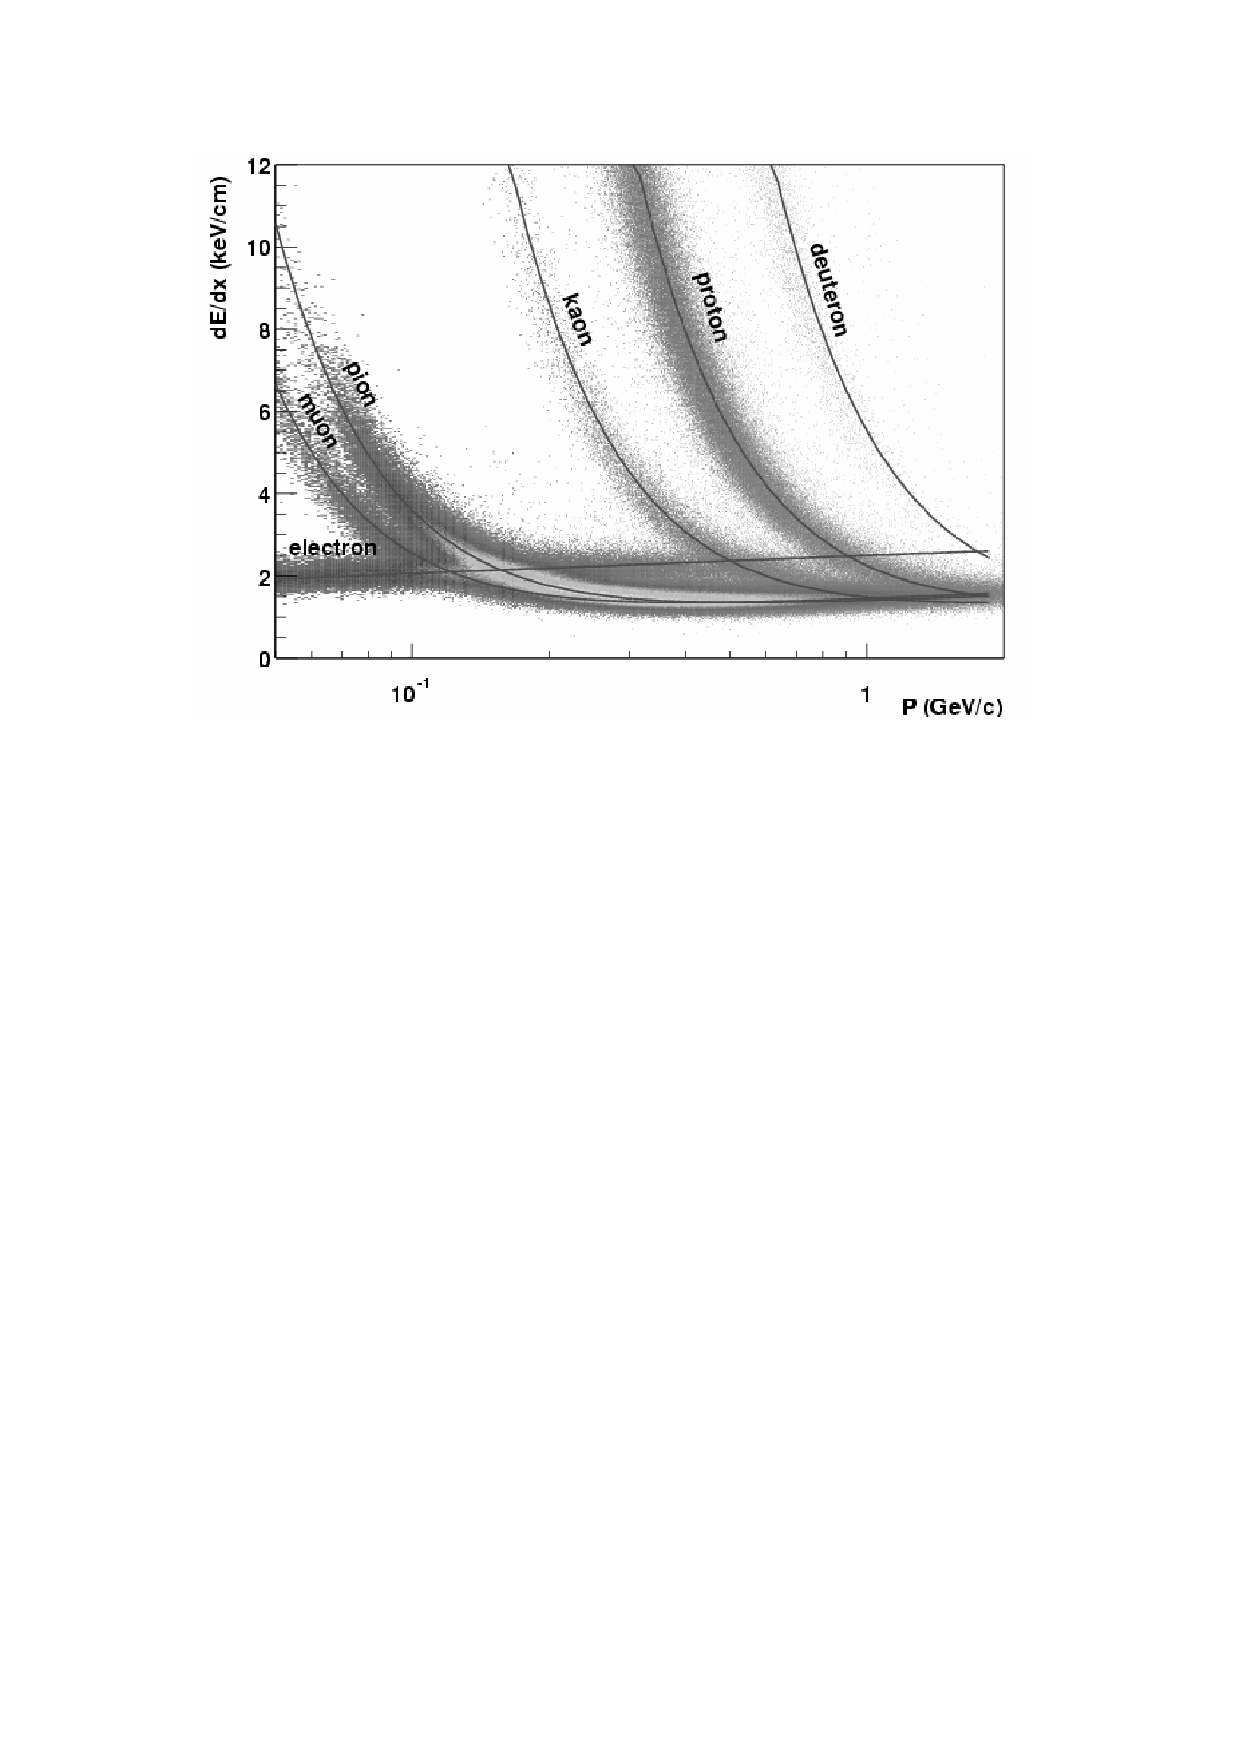
\includegraphics[scale=1.0]{Plots/Detector/TPC_dedx.pdf}
\end{center}
\caption[Ionization Energy Loss in TPC]{Ionization energy loss of tracks in the STAR TPC. Labeled bands show how the $dE/dx$ measurement can be used for particle identification~\cite{tpcNIM}.}
\label{fig:TPC_dedx}
\end{figure}

\begin{figure}[htbp]
\begin{center}
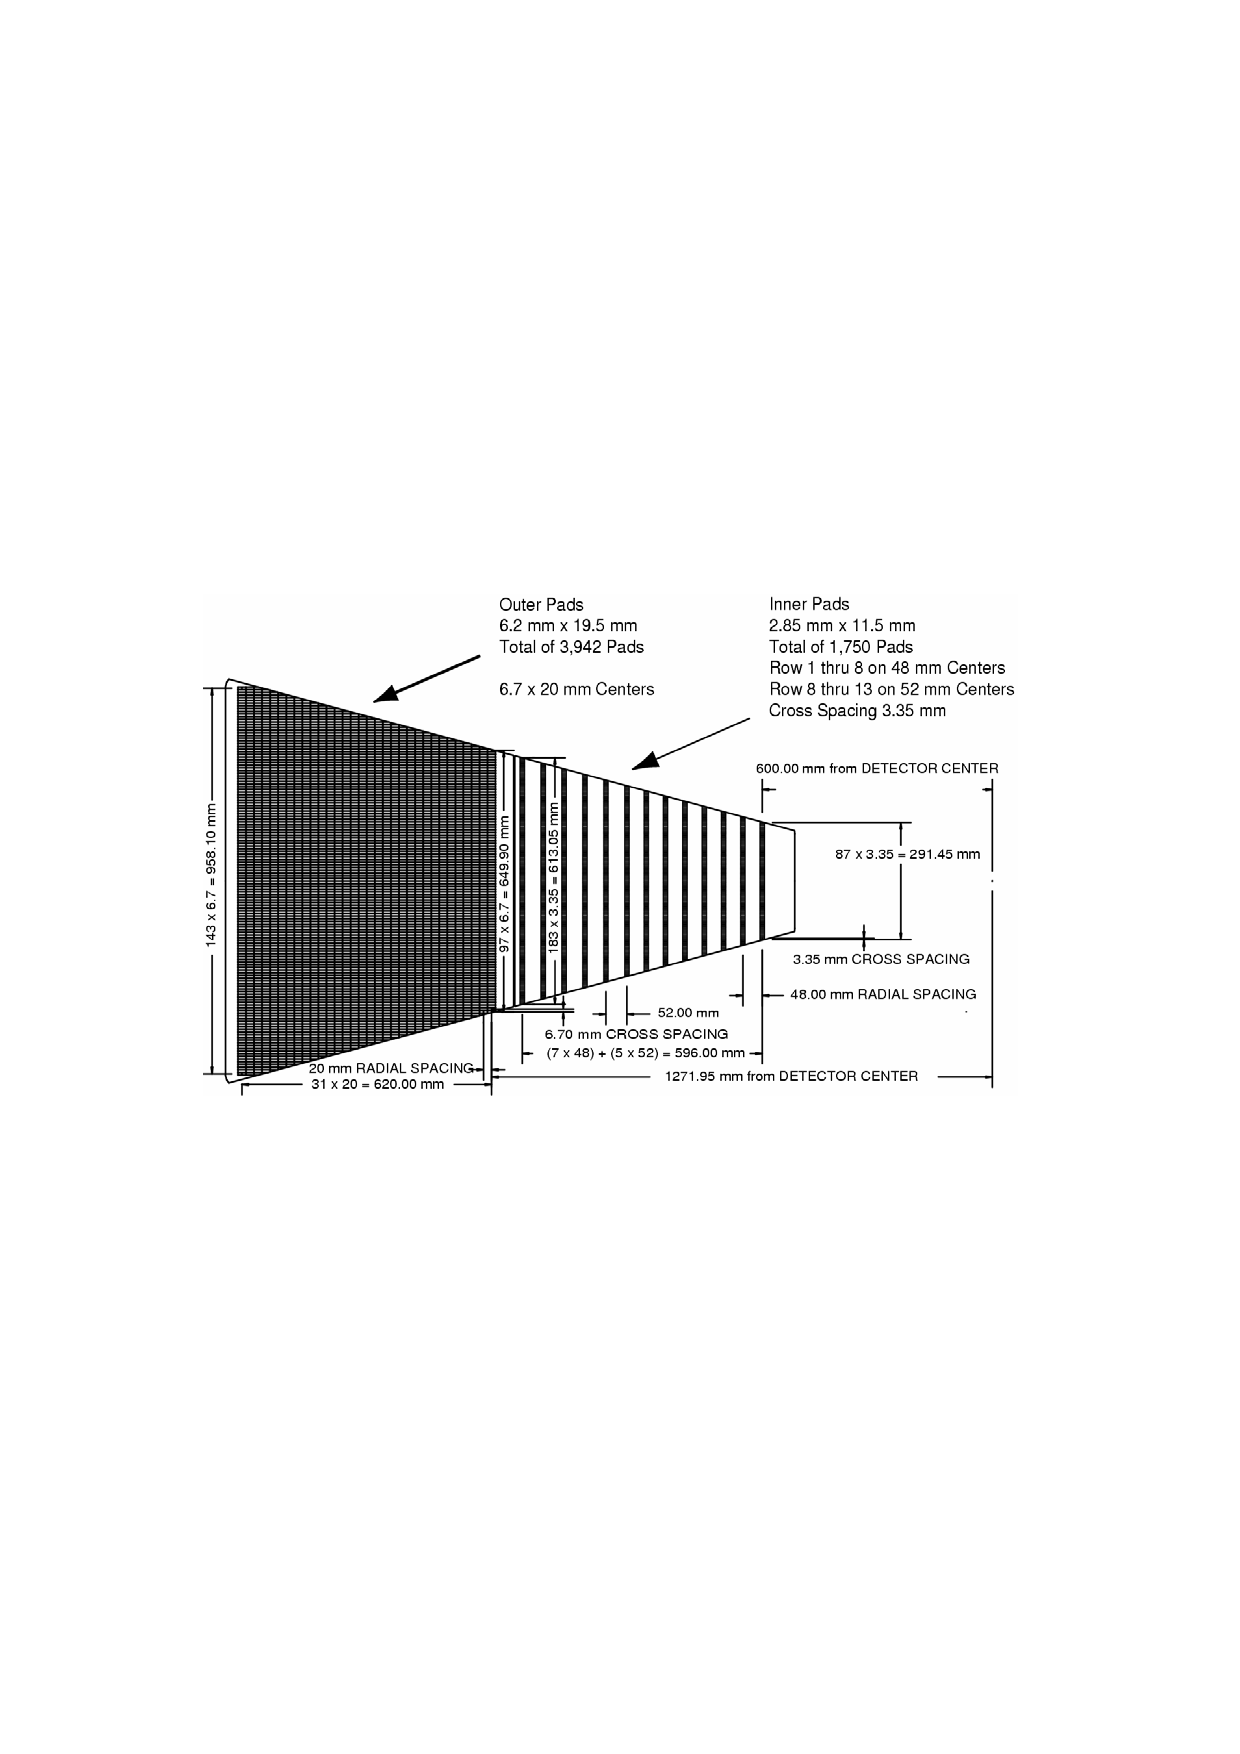
\includegraphics[scale=1.0]{Plots/Detector/TPC_pad.pdf}
\end{center}
\caption[TPC Sector]{Schematic of one TPC pad plane. The difference in spacing between inner and outer pads can be seen~\cite{tpcNIM}.}
\label{fig:TPC_pad}
\end{figure}

\section{Barrel Electromagnetic Calorimeter}

The Barrel Electromagnetic Calorimeter (BEMC) is a lead-scintillator sampling calorimeter located outside of the TPC, the tower assemblies are within the coil of the main STAR magnet but the readout PMTs are located outside. The BEMC is used for studying high $\pt$ processes such as jets, direct $\gamma$'s, and electrons from heavy meson decays. The calorimeter, being one of the fastest systems in STAR, is also used in triggering on high transverse energy. There are two main subsystems of the BEMC: the towers of lead and scintillator, which produce the particle showers and collect the light to measure the energy, and the Shower Maximum Detector (SMD) for measuring the profile of showers in the BEMC which can be used to select electromagnetic showers such as those caused by electrons and photons~\cite{emcNIM}.

\subsection{EMC Towers}

The towers of the BEMC cover $2\pi$ in azimuth and have coverage from -1 to 1 in $\eta$. The inner surface of the calorimeter sits approximately 2.2 m from the beam line in STAR. The towers are grouped into modules which each cover $6\degree$ in $\phi$ and 1 in $\Delta\eta$. There are in total 120 modules, 60 on each half (lengthwise) of the detector. Each tower consists of alternating layers of lead and scintillator. There are 21 scintillating layers and 20 lead layers in each tower, the tower depth is approximately 20 radiation lengths. The towers have a projective geometry so that towers located farther out from $\eta = 0$ still point back to the center of the interaction region in STAR. Figure~\ref{fig:BEMC_towera} shows the structure and dimensions of a single tower from near the center of the BEMC ($\eta \approx 0$). In Figure~\ref{fig:BEMC_towerb} is a photograph of a single BEMC module. The left end is near $\eta = 0$ and the projective geometry of the towers can be seen when moving right along the modules.

\begin{figure}[htbp]
	\begin{subfigure}{0.5\textwidth}
		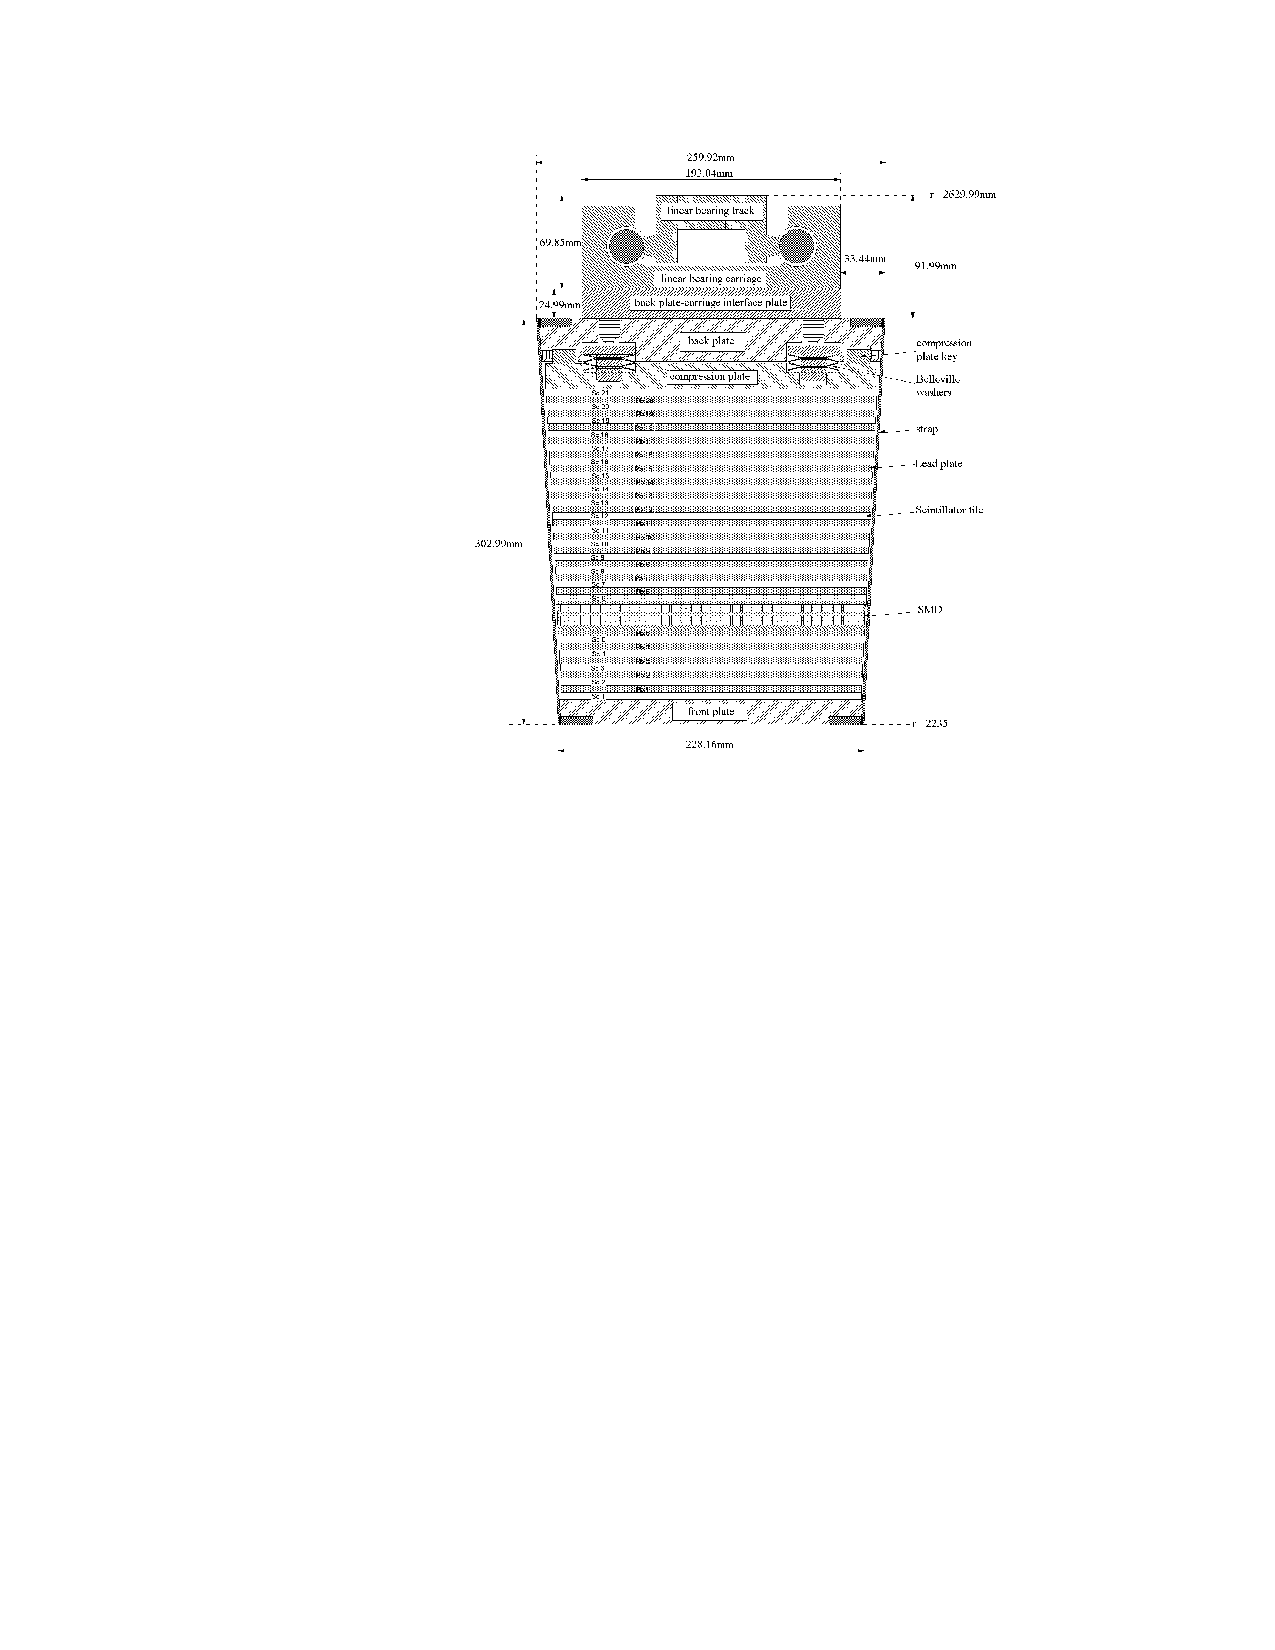
\includegraphics[width=\textwidth]{Plots/Detector/BEMC_tower.pdf}
		\caption{BEMC Tower Diagram}
		\label{fig:BEMC_towera}
	\end{subfigure}
	\begin{subfigure}{0.5\textwidth}
		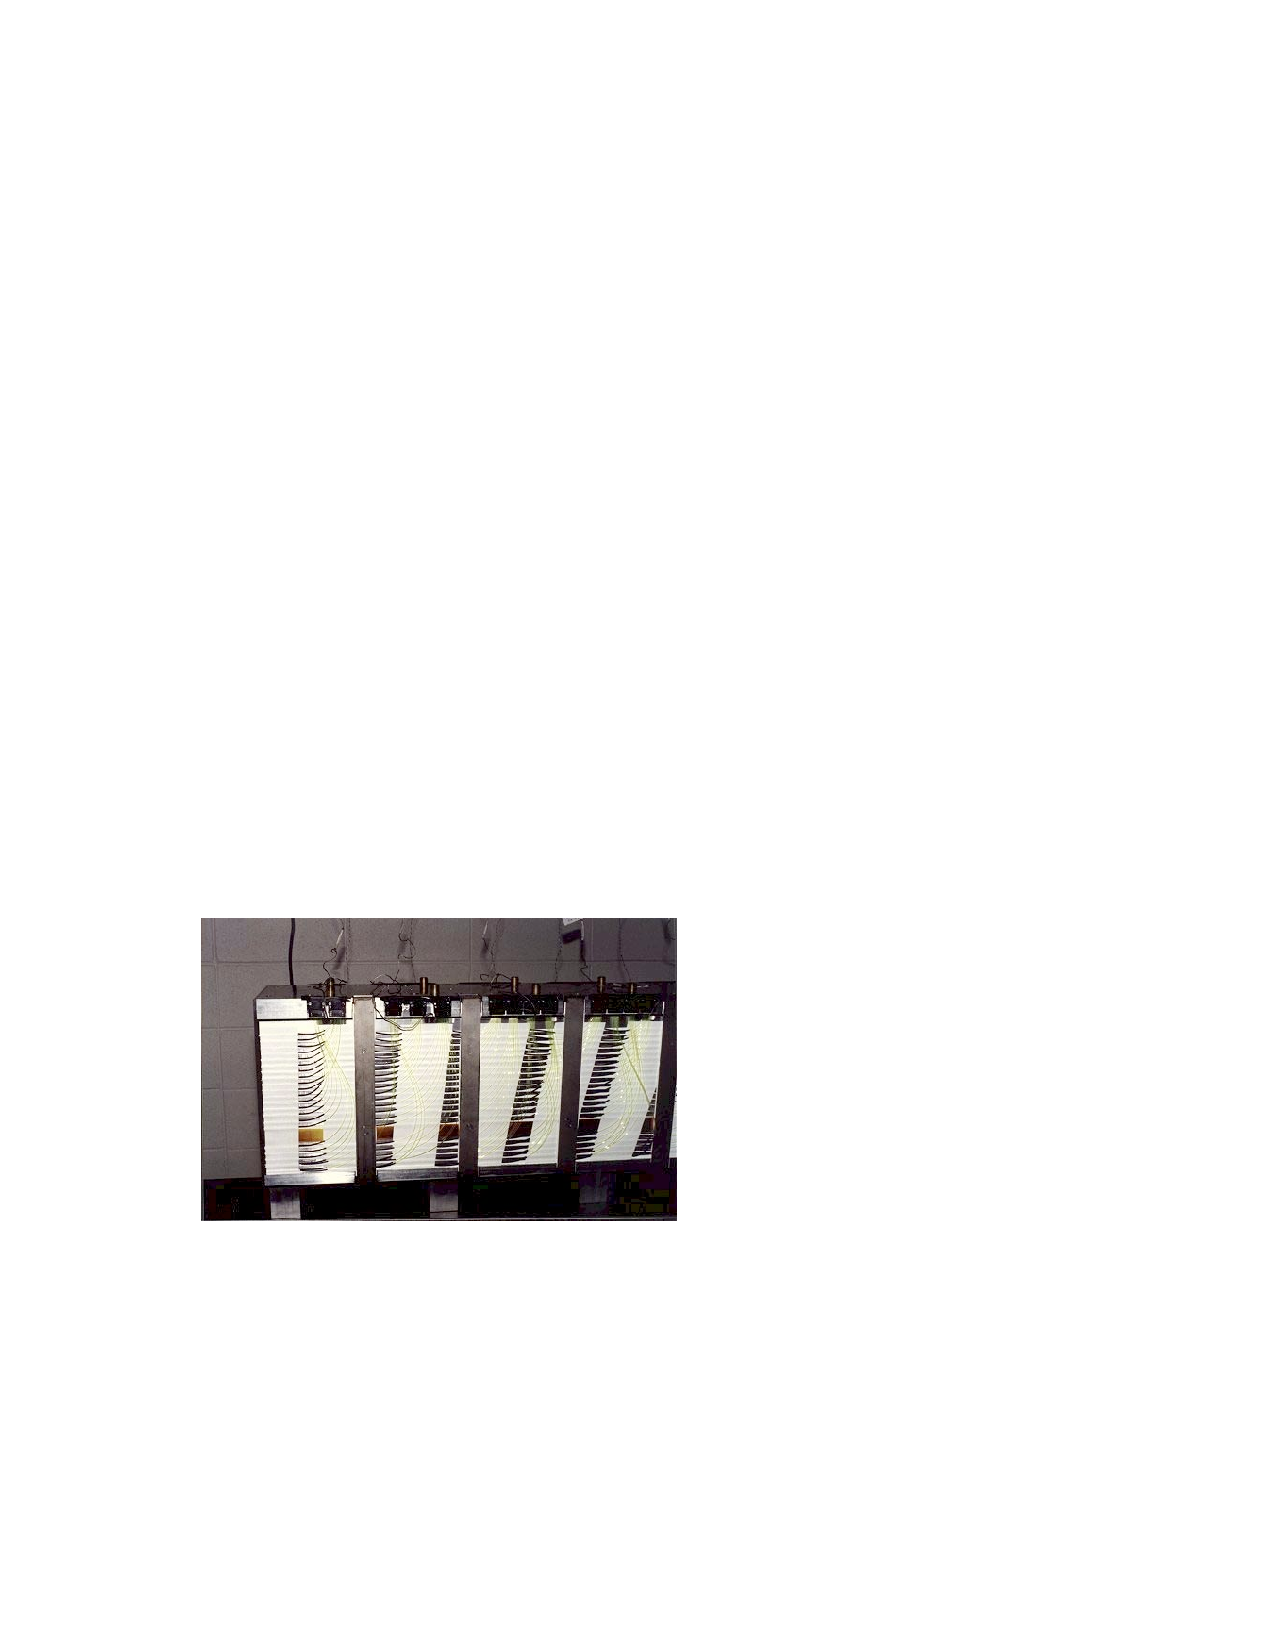
\includegraphics[width=\textwidth]{Plots/Detector/BEMC_proj.pdf}
		\caption{BEMC Module}
		\label{fig:BEMC_towerb}
	\end{subfigure}
\caption[BEMC Towers]{Left figure is a diagram of one BEMC tower as seen from the side. The location of the SMD is indicated after the fifth lead layer. Right shows a photograph of a single BEMC module showing the projective geometry of the towers~\cite{emcNIM}.}
\label{fig:BEMC_tower}
\end{figure}

Particle showers in the BEMC towers produce light in the scintillating layers which is then collected and read out by a wavelength shifting fiber. The fibers run from each scintillating layer of the tower to a photomultiplier tube (one per tower) located outside the STAR magnet.

\subsection{Shower Maximum Detector}

The Shower Maximum Detector (SMD) is located within the BEMC towers and provides finer positional resolution than the BEMC towers alone, allowing us to study the profile and development of showers inside the BEMC. As shown in Figure~\ref{fig:BEMC_towera} the BSMD sits after the fifth lead layer in the tower, which corresponds to $\approx 5.6 X_{0}$ of material total in STAR in front of the SMD. The SMD itself is a wire proportional detector with strip readout, there are two perpendicular directions for the chambers to measure shower profiles in both $\eta$ and $\phi$. The strips are $\approx 1.5$ cm in both directions for $|\eta| < .5$ and 1.88 cm in the $\eta$ direction outside of that. For electrons with $\pt > 1$ GeV/c the SMD is near the depth of widest shower development (the Moliere radius for lead is $\approx 3.2$ cm), however for hadrons the depth of maximum development is around 1 nuclear interaction length, which for the BEMC close to the entire length of one BEMC tower. Thus we can use the width of showers in the SMD as a powerful tool for rejecting showers from hadrons or minimum ionizing particles. Figure~\ref{fig:SMD} shows how the SMD works in practice, an electron enters the detector, develops into a wide shower and registers multiple hits in the SMD strips in both directions. The SMD, in addition to profiling showers, also gives much better position resolution for the center position of showers within the BEMC. At the front plane of the SMD the position resolution is $\sigma = 2.4 \text{ mm} + 5.6 \text{ mm}/\sqrt{E}$ GeV. Tracks from the TPC point to the SMD with millimeter precision and thus we can use spatial matching of tracks in the BEMC and the TPC to further improve electron identification.

\begin{figure}[htbp]
\begin{center}
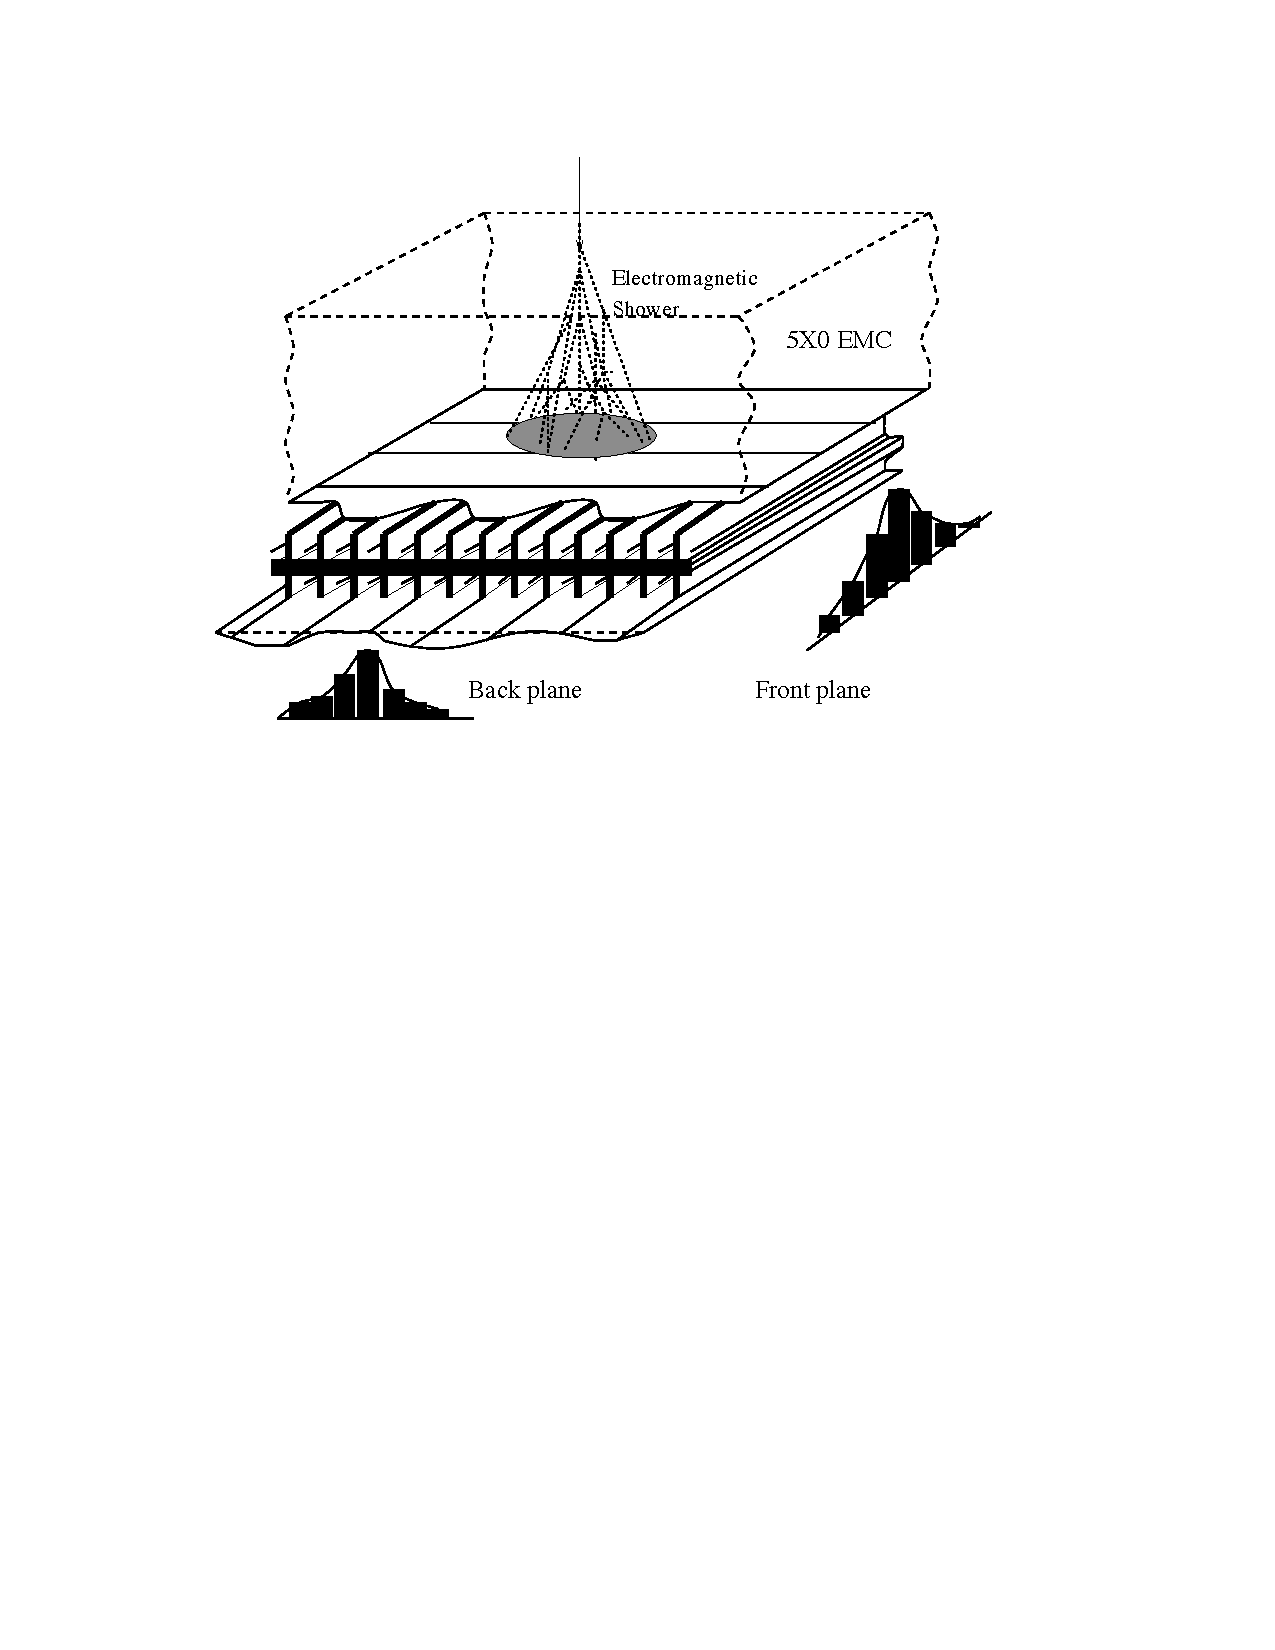
\includegraphics[scale=1.0]{Plots/Detector/SMD.pdf}
\end{center}
\caption[BSMD Diagram]{Illustration of the function of the BSMD detector. Particle enters the tower (at top) and develops into a shower which registers hits in the $\eta$ and $\phi$ directions in the BSMD~\cite{emcNIM}.}
\label{fig:SMD}
\end{figure}
